%%%%%%%%%%%%%%%%%%%%%%%%%%%%%%%%%%%%

\section{直線の当てはめ、残差、相関}

%%%%%%%%%%%%%%%%%%%%%%%%%%%%%%%%%%%%

\subsection{データへの直線の当てはめ}

%%%%%%%%%%%%%%%%%%%%%%%%%%%%%%%%%%%%

\begin{frame}
\frametitle{数値変数のモデル化}

本節では、2つの数値変数間の関係を定量化する方法と、数値または質的な説明変数を用いて数値の目的変数をモデル化する方法を学ぶ。

\end{frame}

%%%%%%%%%%%%%%%%%%%%%%%%%%%%%%%%%%%%

\begin{frame}
\frametitle{貧困率と高校卒業率}

下の\hl{散布図}は、米国全50州とワシントンDCの高校卒業率と、貧困ライン（2012年時点で4人家族の年収23,050ドル未満）以下で生活する住民の割合との関係を示している。

\twocol{0.55}{0.45}{
\begin{center}
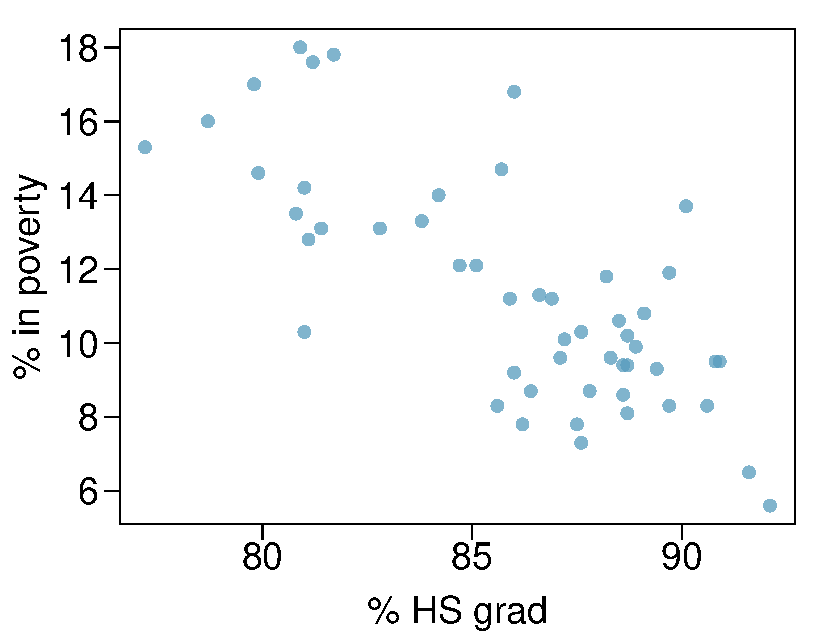
\includegraphics[width=\textwidth]{8-1_linefit_res_corr/figures/poverty/poverty_hsgrad}
\end{center}
}
{
\dq{目的変数は？}
\soln{貧困率（\%）}
\dq{説明変数は？}
\soln{高校卒業率（\%）}
\dq{関係は？}
\soln{線形、負の相関、中程度の強さ}
}

\end{frame}

%%%%%%%%%%%%%%%%%%%%%%%%%%%%%%%%%%%

\subsection{線形回帰を用いた貧困率の予測}

%%%%%%%%%%%%%%%%%%%%%%%%%%%%%%%%%%%

\begin{frame}

米国の高校卒業率から貧困率を予測する線形モデルは次のとおりである：

\[ \hat{poverty} = 64.78 - 0.62 \times HS_{grad} \]

「ハット（$\hat{\:}$）」は推定値であることを示す。

\end{frame}

%%%%%%%%%%%%%%%%%%%%%%%%%%%%%%%%%%%

\begin{frame}

\dq{ジョージア州の高校卒業率は85.1\%である。このモデルは同州の貧困率をどのように予測するか？}

\[ 64.78 - 0.62 \times 85.1 = 12.018 \]

\end{frame}

%%%%%%%%%%%%%%%%%%%%%%%%%%%%%%%%%%%

\subsection{直線の目視確認}

%%%%%%%%%%%%%%%%%%%%%%%%%%%%%%%%%%%

\begin{frame}
\frametitle{直線の目視確認}

\twocol{0.3}{0.7}
{
\pq{貧困率と高校卒業率の線形関係に最もよく当てはまる直線はどれか。1つ選べ。}
\soln{\only<2>{\orange{
(a)
}}}
}
{
\begin{center}

\includegraphics[width=\textwidth]{8-2_least_square_reg/figures/poverty/poverty_hsgrad_manylines}
\end{center}
}
\end{frame}

%%%%%%%%%%%%%%%%%%%%%%%%%%%%%%%%%%%

\subsection{残差}

%%%%%%%%%%%%%%%%%%%%%%%%%%%%%%%%%%%

\begin{frame}
\frametitle{残差}

\hl{残差}とはモデルの当てはめから残ったものである：データ = 当てはめ値 + 残差

\begin{center}
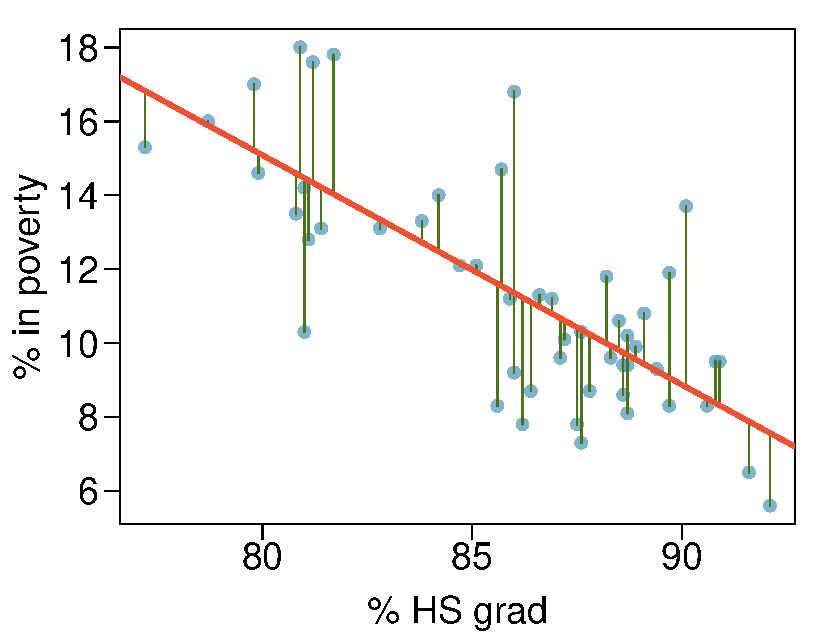
\includegraphics[width=0.8\textwidth]{8-2_least_square_reg/figures/poverty/poverty_hsgrad_res}
\end{center}

\end{frame}

%%%%%%%%%%%%%%%%%%%%%%%%%%%%%%%%%%

\begin{frame}
\frametitle{残差（続き）}

\formula{残差}{
残差は観測値（$y_i$）と予測値$\hat{y}_i$との差である。
\[ e_i = y_i - \hat{y}_i \]
}
\vspace{-0.5cm}
\twocol{0.6}{0.4}
{
\begin{center}
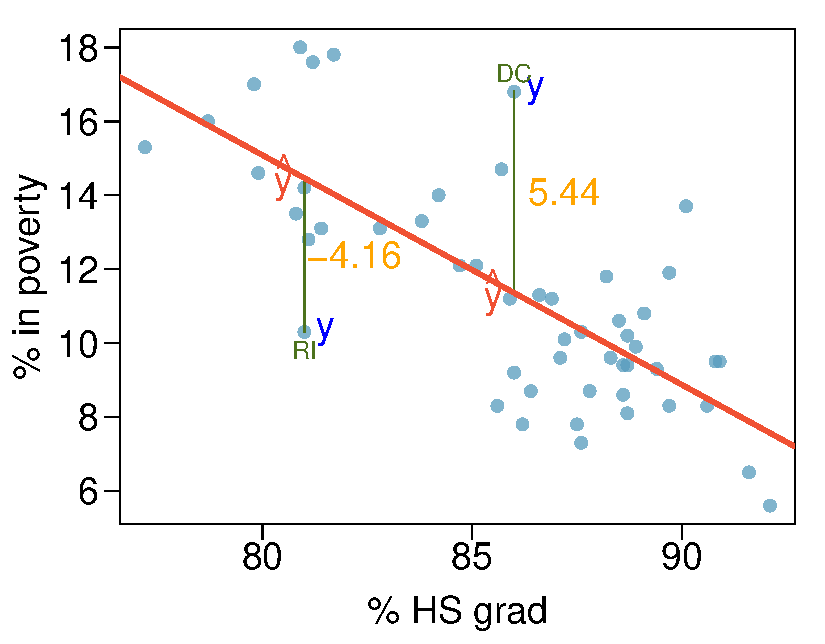
\includegraphics[width=\textwidth]{8-2_least_square_reg/figures/poverty/poverty_hsgrad_res_text}
\end{center}
}
{
\begin{itemize}
\item ワシントンDCの貧困率は予測値より5.44\%高い。
\item ロードアイランド州の貧困率は予測値より4.16\%低い。
\end{itemize}
}


\end{frame}

%%%%%%%%%%%%%%%%%%%%%%%%%%%%%%%%%%

\subsection{相関による線形関係の記述}

%%%%%%%%%%%%%%%%%%%%%%%%%%%%%%%%%%%

\begin{frame}
\frametitle{関係の定量化}

\begin{itemize}

\item \hl{相関}は2つの変数間の\orange{線形}な関連の強さを表す。

\item $-1$（完全な負の相関）から$+1$（完全な正の相関）の値をとる。

\item 値が0の場合、線形な関連がないことを示す。

\end{itemize}

\end{frame}

%%%%%%%%%%%%%%%%%%%%%%%%%%%%%%%%%%%

\begin{frame}
\frametitle{相関の推測}

\pq{貧困率と高校卒業率の相関として最もよい推測はどれか？}
\twocol{0.4}{0.6}
{
\begin{enumerate}[(a)]
\item 0.6
\solnMult{-0.75}
\item -0.1
\item 0.02
\item -1.5
\end{enumerate}
}
{
\begin{center}
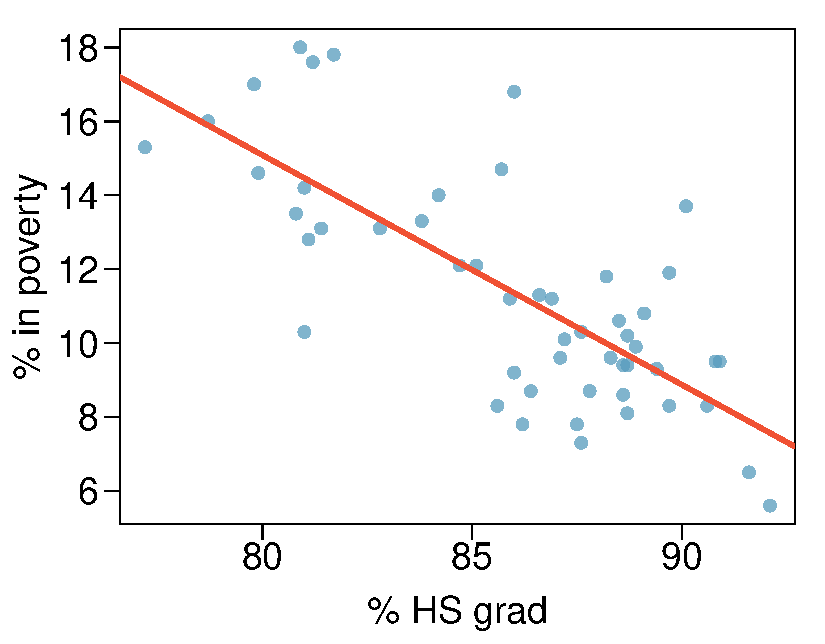
\includegraphics[width=\textwidth]{8-1_linefit_res_corr/figures/poverty/poverty_hsgrad_line}
\end{center}
}

\end{frame}

%%%%%%%%%%%%%%%%%%%%%%%%%%%%%%%%%%

\begin{frame}
\frametitle{相関の推測}

\pq{貧困率と「夫なし女性世帯主」の割合の相関として最もよい推測はどれか？}

\twocol{0.4}{0.6}
{
\begin{enumerate}[(a)]
\item 0.1
\item -0.6
\item -0.4
\item 0.9
\solnMult{0.5}
\end{enumerate}
}
{
\begin{center}
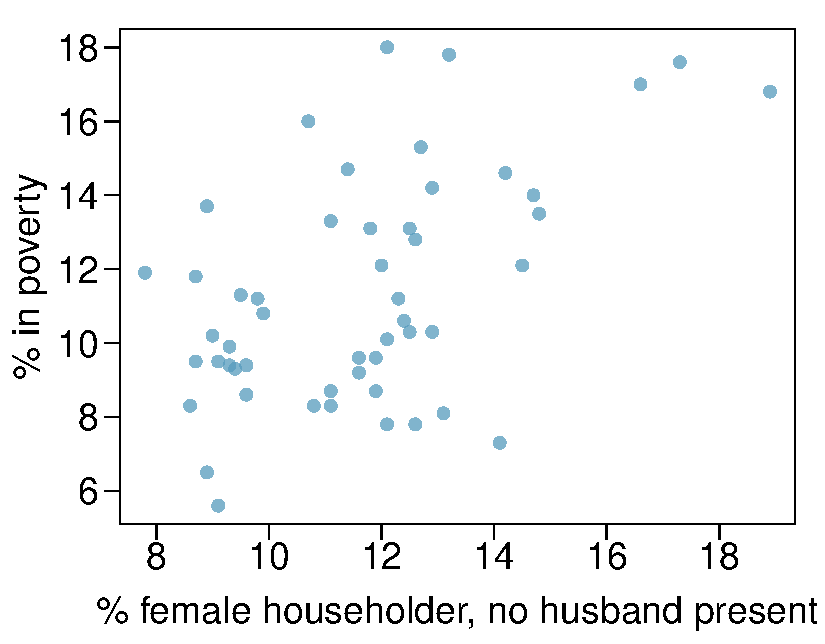
\includegraphics[width=\textwidth]{8-1_linefit_res_corr/figures/poverty/poverty_nohusband}
\end{center}
}

\end{frame}

%%%%%%%%%%%%%%%%%%%%%%%%%%%%%%%%%%

\begin{frame}
\frametitle{相関の評価}

\pq{以下のうち、最も強い相関（相関係数が+1または-1に最も近い）を持つのはどれか？}

\twocol{0.8}{0.2}
{
\begin{center}
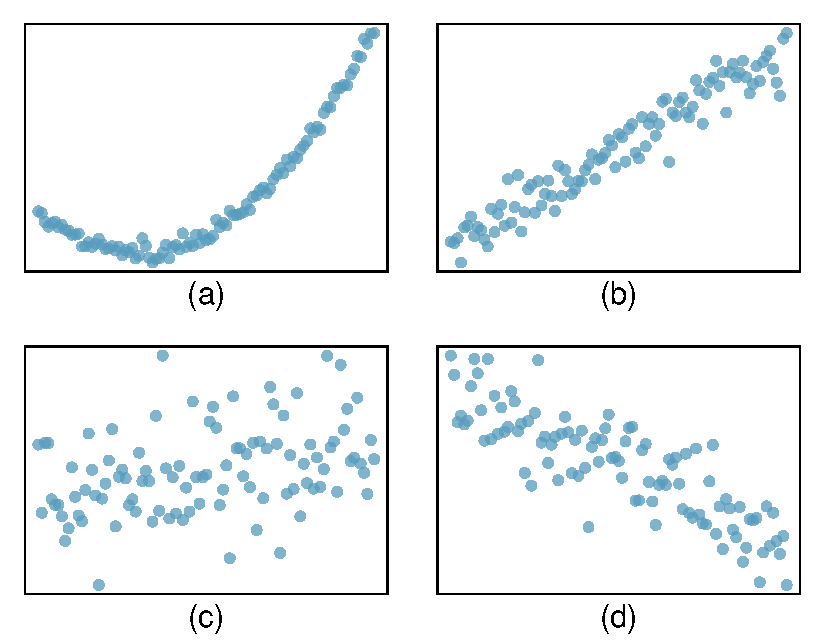
\includegraphics[width=0.75\textwidth]{8-1_linefit_res_corr/figures/cor/cor}
\end{center}
}
{
\soln{\only<2>{\orange{
(b) $\rightarrow$ 相関は\underline{線形}な関連を意味する
}}}
}

\end{frame}
